\section{Domain Model}
\label{sec:domain-model}

Fig.~\ref{fig:domain-model} presents the conceptual domain model for the Reading the Reader platform.
The model identifies the principal entities in the problem domain, their key attributes, and the associations between them, expressed at the analysis level without reference to any implementation structure.
It establishes the shared vocabulary that grounds the functional requirements stated in Sec.~\ref{sec:functional-requirements}.

\begin{figure}[htbp]
\centering
\resizebox{0.97\linewidth}{!}{%
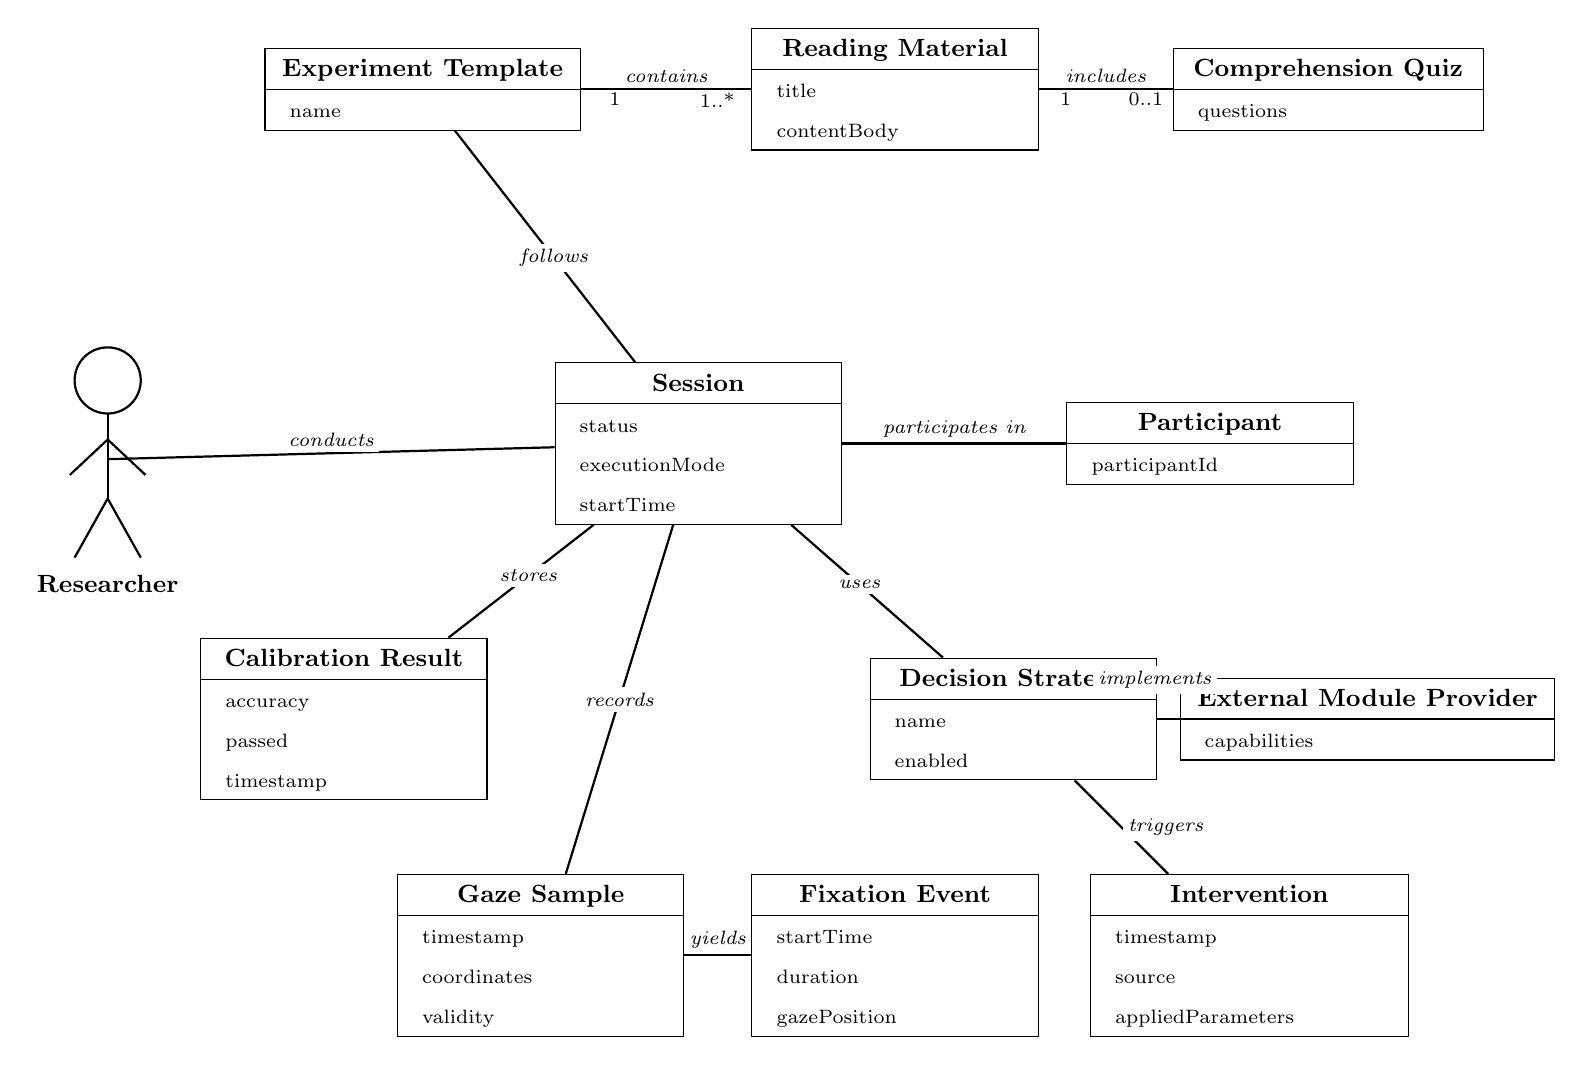
\begin{tikzpicture}[
  assoc/.style={draw, thick},
  lbl/.style={font=\scriptsize\itshape, fill=white, inner sep=2pt},
  mult/.style={font=\scriptsize, fill=white, inner sep=1pt}
]

%% ── Entities ──────────────────────────────────────────────────────────────────
%% Each entity is a node containing a two-compartment tabular:
%% upper compartment = entity name (centred, bold),
%% lower compartment = attributes (left-aligned, scriptsize).

% ── Content hierarchy (top band) ─────────────────────────────────────────────

\node[inner sep=0, outer sep=0] (template) at (-3.5, 11.0) {%
  \renewcommand{\arraystretch}{1.2}%
  \begin{tabular}{|p{3.2cm}|}
  \hline
  \multicolumn{1}{|c|}{\small\bfseries Experiment Template}\\
  \hline
  \scriptsize\ name\\
  \hline
  \end{tabular}};

\node[inner sep=0, outer sep=0] (material) at (2.5, 11.0) {%
  \renewcommand{\arraystretch}{1.2}%
  \begin{tabular}{|p{3.2cm}|}
  \hline
  \multicolumn{1}{|c|}{\small\bfseries Reading Material}\\
  \hline
  \scriptsize\ title\\
  \scriptsize\ contentBody\\
  \hline
  \end{tabular}};

\node[inner sep=0, outer sep=0] (quiz) at (8.0, 11.0) {%
  \renewcommand{\arraystretch}{1.2}%
  \begin{tabular}{|p{3.5cm}|}
  \hline
  \multicolumn{1}{|c|}{\small\bfseries Comprehension Quiz}\\
  \hline
  \scriptsize\ questions\\
  \hline
  \end{tabular}};

% ── Session core (middle band) ────────────────────────────────────────────────

% Researcher drawn as UML actor (stick figure)
\def\rX{-7.5} \def\rY{5.3}
\draw[thick] (\rX,      \rY+2.0)  circle (0.42);
\draw[thick] (\rX,      \rY+1.58) -- (\rX,       \rY+0.5);
\draw[thick] (\rX,      \rY+0.5)  -- (\rX-0.42,  \rY-0.25);
\draw[thick] (\rX,      \rY+0.5)  -- (\rX+0.42,  \rY-0.25);
\draw[thick] (\rX,      \rY+1.25) -- (\rX-0.48,  \rY+0.80);
\draw[thick] (\rX,      \rY+1.25) -- (\rX+0.48,  \rY+0.80);
\node[font=\small\bfseries, align=center, below] at (\rX, \rY-0.35) {Researcher};
\coordinate (researcher) at (\rX, \rY+1.0);

\node[inner sep=0, outer sep=0] (session) at (0.0, 6.5) {%
  \renewcommand{\arraystretch}{1.2}%
  \begin{tabular}{|p{3.2cm}|}
  \hline
  \multicolumn{1}{|c|}{\small\bfseries Session}\\
  \hline
  \scriptsize\ status\\
  \scriptsize\ executionMode\\
  \scriptsize\ startTime\\
  \hline
  \end{tabular}};

\node[inner sep=0, outer sep=0] (participant) at (6.5, 6.5) {%
  \renewcommand{\arraystretch}{1.2}%
  \begin{tabular}{|p{3.2cm}|}
  \hline
  \multicolumn{1}{|c|}{\small\bfseries Participant}\\
  \hline
  \scriptsize\ participantId\\
  \hline
  \end{tabular}};

% ── Strategy and calibration (lower-middle band) ──────────────────────────────

\node[inner sep=0, outer sep=0] (calibration) at (-4.5, 3.0) {%
  \renewcommand{\arraystretch}{1.2}%
  \begin{tabular}{|p{3.2cm}|}
  \hline
  \multicolumn{1}{|c|}{\small\bfseries Calibration Result}\\
  \hline
  \scriptsize\ accuracy\\
  \scriptsize\ passed\\
  \scriptsize\ timestamp\\
  \hline
  \end{tabular}};

\node[inner sep=0, outer sep=0] (strategy) at (4.0, 3.0) {%
  \renewcommand{\arraystretch}{1.2}%
  \begin{tabular}{|p{3.2cm}|}
  \hline
  \multicolumn{1}{|c|}{\small\bfseries Decision Strategy}\\
  \hline
  \scriptsize\ name\\
  \scriptsize\ enabled\\
  \hline
  \end{tabular}};

\node[inner sep=0, outer sep=0] (provider) at (8.5, 3.0) {%
  \renewcommand{\arraystretch}{1.2}%
  \begin{tabular}{|p{3.6cm}|}
  \hline
  \multicolumn{1}{|c|}{\small\bfseries External Module Provider}\\
  \hline
  \scriptsize\ capabilities\\
  \hline
  \end{tabular}};

% ── Event data (bottom band) ──────────────────────────────────────────────────

\node[inner sep=0, outer sep=0] (gaze) at (-2.0, 0.0) {%
  \renewcommand{\arraystretch}{1.2}%
  \begin{tabular}{|p{3.2cm}|}
  \hline
  \multicolumn{1}{|c|}{\small\bfseries Gaze Sample}\\
  \hline
  \scriptsize\ timestamp\\
  \scriptsize\ coordinates\\
  \scriptsize\ validity\\
  \hline
  \end{tabular}};

\node[inner sep=0, outer sep=0] (fixation) at (2.5, 0.0) {%
  \renewcommand{\arraystretch}{1.2}%
  \begin{tabular}{|p{3.2cm}|}
  \hline
  \multicolumn{1}{|c|}{\small\bfseries Fixation Event}\\
  \hline
  \scriptsize\ startTime\\
  \scriptsize\ duration\\
  \scriptsize\ gazePosition\\
  \hline
  \end{tabular}};

\node[inner sep=0, outer sep=0] (intervention) at (7.0, 0.0) {%
  \renewcommand{\arraystretch}{1.2}%
  \begin{tabular}{|p{3.6cm}|}
  \hline
  \multicolumn{1}{|c|}{\small\bfseries Intervention}\\
  \hline
  \scriptsize\ timestamp\\
  \scriptsize\ source\\
  \scriptsize\ appliedParameters\\
  \hline
  \end{tabular}};

%% ── Associations ──────────────────────────────────────────────────────────────

% Actors <-> Session
\draw[assoc] (researcher)  -- node[lbl, above] {conducts}        (session);
\draw[assoc] (participant) -- node[lbl, above] {participates in} (session);

% Session follows ExperimentTemplate
\draw[assoc] (session) -- node[lbl, fill=white, pos=0.45] {follows} (template);

% Content hierarchy
\draw[assoc] (template) --
  node[lbl, above]           {contains}
  node[mult, below, pos=0.2] {1}
  node[mult, below, pos=0.8] {1..*}
  (material);

\draw[assoc] (material) --
  node[lbl, above]           {includes}
  node[mult, below, pos=0.2] {1}
  node[mult, below, pos=0.8] {0..1}
  (quiz);

% Session stores CalibrationResult
\draw[assoc] (session) -- node[lbl, fill=white, pos=0.45] {stores} (calibration);

% Session uses DecisionStrategy
\draw[assoc] (session) -- node[lbl, fill=white, pos=0.45] {uses}   (strategy);

% ExternalModuleProvider implements DecisionStrategy
\draw[assoc] (provider) -- (strategy);
\node[lbl] at (5.8, 3.5) {implements};

% Session records GazeSample
\draw[assoc] (session) -- node[lbl, fill=white, pos=0.5] {records} (gaze);

% GazeSample yields FixationEvent
\draw[assoc] (gaze) -- node[lbl, above] {yields} (fixation);

% DecisionStrategy triggers Intervention
\draw[assoc] (strategy) -- node[lbl, right] {triggers} (intervention);

\end{tikzpicture}%
}
\caption{%
Conceptual domain model for the Reading the Reader platform.
Each box shows the entity name and its analysis-level attributes.
Lines represent associations labelled with the nature of the relationship;
multiplicity notation follows UML convention.
The Researcher is shown as a UML actor because it represents a human role
with no data attributes at this level of analysis.%
}
\label{fig:domain-model}
\end{figure}

The model centres on \textbf{Session}, the primary unit of experimental activity,
which carries the execution mode and status that determine how the session
is conducted.
A session is associated with one \textbf{Researcher} and one \textbf{Participant}
(identified by a \textit{participantId}) and follows a predefined
\textbf{Experiment Template} that specifies an ordered set of
\textbf{Reading Materials}.
Each reading material carries a title and a content body, and may include
an optional \textbf{Comprehension Quiz} with its associated questions.
Before a session begins, calibration is performed and the outcome is stored as
a \textbf{Calibration Result}, recording accuracy, pass or fail status, and a
timestamp.
During the session, the eye tracker produces \textbf{Gaze Samples} carrying
timestamped coordinates and a validity flag; the analysis layer yields
\textbf{Fixation Events} from these samples.
A \textbf{Decision Strategy} (characterised by a name and an enabled flag)
observes the incoming events and triggers \textbf{Interventions}, each recorded
with a timestamp, the source that triggered it, and the parameters applied.
An \textbf{External Module Provider} may fulfil the strategy role by connecting
to the platform and declaring its capabilities through the integration interface.
